
\subsection{Answers}
\begin{table}[htb]%
\begin{center}%
\caption{Q10: How did you learn MPI?}%
\label{tab:Q10-ans}%
\begin{tabular}{l|l|r}%
\hline%
Choice & Abbrv. & \# Answers \\%
\hline%
I read the MPI standard document. & Standard & 329 (38.8\%) \\%
I had lecture(s) at school. & School & 294 (34.7\%) \\%
I read articles found on Internet. & Internet & 439 (51.8\%) \\%
I read book(s). & Books & 283 (33.4\%) \\%
{\small Other lectures or tutorials (workplace, $\cdots$} & Other & 438 (51.7\%) \\%
I have not learned MPI. & Never learned & 26 (3.1\%) \\%
other & - & 51 (6.0\%) \\%
\hline%
\multicolumn{2}{c}{total} & 1860 (847)\\%
\hline%
\end{tabular}%
\end{center}%
\end{table}%

\clearpage%
{\footnotesize\begin{landscape}%
\begin{longtable}[htb]{r|c|c|c|c|c|c|c|c|c|c}%
\caption{Q10: How did you learn MPI?}%
\label{tab:Q10-mans} \\%
\hline%
Multi-Answer & overall & FR & GR & IT & UK & eu & JP & RU & US & others \\
 \hline%
\endfirsthead%
\multicolumn{11}{r}{(continued from the previous page)}\\%
\hline%
Multi-Answer & overall & FR & GR & IT & UK & eu & JP & RU & US & others \\
 \hline%
\endhead%
\hline%
(total) & 847 & 124 & 158 & 57 & 66 & 144 & 64 & 94 & 57 & 83 \\%
\hline%
\multicolumn{11}{r}{(continue to the next page)}\\%
\endfoot%
\hline%
(total) & 847 & 124 & 158 & 57 & 66 & 144 & 64 & 94 & 57 & 83 \\%
\hline%
\endlastfoot%
\hline%
{Other lec.} & 67 & 11 & 18 & 10 & 8 & 7 & 2 & 2 & 3 & 6 \\%
{Internet} & 63 & 10 & 11 & 4 & 2 & 8 & 3 & 7 & 1 & 17 \\%
{Other lec., Internet} & 55 & 7 & 15 & 5 & 5 & 6 & 5 & 7 & 2 & 3 \\%
{School} & 40 & 8 & 5 & 7 & 2 & 10 & 4 & 2 & 1 & 1 \\%
{Standard, Other lec.} & 40 & 8 & 9 & 4 & 1 & 5 & 0 & 8 & 2 & 3 \\%
{School, Internet} & 36 & 5 & 5 & 0 & 4 & 7 & 0 & 8 & 3 & 4 \\%
{School, Other lec., Internet} & 34 & 9 & 4 & 3 & 4 & 6 & 3 & 4 & 0 & 1 \\%
{Standard, Other lec., Internet} & 31 & 2 & 16 & 1 & 3 & 4 & 2 & 1 & 0 & 2 \\%
{Books, Internet} & 28 & 4 & 5 & 2 & 3 & 3 & 3 & 1 & 2 & 5 \\%
{Standard} & 27 & 3 & 4 & 2 & 0 & 4 & 9 & 4 & 1 & 0 \\%
{Books} & 26 & 3 & 1 & 0 & 1 & 1 & 5 & 3 & 4 & 8 \\%
{Standard, Internet} & 24 & 6 & 5 & 0 & 1 & 3 & 2 & 2 & 3 & 2 \\%
{Standard, Books} & 23 & 1 & 2 & 2 & 0 & 4 & 3 & 6 & 4 & 1 \\%
{Books, School, Other lec.} & 23 & 3 & 2 & 1 & 1 & 9 & 2 & 1 & 1 & 3 \\%
{School, Other lec.} & 23 & 5 & 2 & 1 & 1 & 7 & 0 & 4 & 1 & 2 \\%
{Standard, Books, Internet} & 22 & 1 & 4 & 0 & 9 & 2 & 2 & 3 & 1 & 0 \\%
{Standard, Books, Other lec., Internet} & 20 & 0 & 4 & 1 & 1 & 4 & 0 & 4 & 1 & 5 \\%
{Books, Other lec., Internet} & 20 & 5 & 1 & 3 & 0 & 4 & 0 & 2 & 2 & 3 \\%
{Books, Other lec.} & 20 & 2 & 2 & 0 & 0 & 6 & 3 & 1 & 4 & 2 \\%
{Standard, School, Internet} & 20 & 4 & 0 & 1 & 1 & 3 & 1 & 9 & 1 & 0 \\%
{Standard, Books, Other lec.} & 19 & 2 & 11 & 2 & 1 & 0 & 1 & 0 & 1 & 1 \\%
{Standard, Books, School, Other lec., Internet} & 18 & 2 & 0 & 2 & 2 & 4 & 2 & 4 & 1 & 1 \\%
{Standard, School, Other lec., Internet} & 18 & 3 & 5 & 0 & 0 & 4 & 1 & 2 & 2 & 1 \\%
{Never learned} & 17 & 2 & 2 & 0 & 0 & 6 & 3 & 1 & 0 & 3 \\%
{Standard, Books, School, Other lec.} & 12 & 1 & 1 & 0 & 0 & 6 & 0 & 1 & 2 & 1 \\%
{Books, School} & 12 & 1 & 1 & 1 & 1 & 0 & 3 & 2 & 2 & 1 \\%
{Standard, School} & 12 & 5 & 1 & 0 & 0 & 2 & 2 & 1 & 0 & 1 \\%
{Books, School, Other lec., Internet} & 11 & 1 & 1 & 1 & 3 & 1 & 1 & 2 & 1 & 0 \\%
{Standard, Books, School} & 10 & 0 & 1 & 1 & 1 & 2 & 0 & 2 & 0 & 3 \\%
{Books, School, Internet} & 8 & 0 & 1 & 0 & 3 & 1 & 1 & 0 & 1 & 1 \\%
{Standard, School, Other lec.} & 7 & 2 & 2 & 0 & 1 & 1 & 0 & 0 & 1 & 0 \\%
{Standard, Books, School, Internet} & 5 & 0 & 2 & 0 & 0 & 0 & 0 & 0 & 2 & 1 \\%
{Other lec., Internet, Never learned} & 2 & 0 & 0 & 0 & 0 & 1 & 0 & 0 & 1 & 0 \\%
{Standard, I read code.} & 2 & 0 & 0 & 0 & 0 & 0 & 0 & 0 & 2 & 0 \\%
{Internet, Never learned} & 2 & 0 & 2 & 0 & 0 & 0 & 0 & 0 & 0 & 0 \\%
{Standard, MPI Forum} & 1 & 0 & 0 & 0 & 0 & 0 & 0 & 0 & 1 & 0 \\%
{Never learned, Stackoverflow, Existing Code} & 1 & 0 & 0 & 0 & 0 & 1 & 0 & 0 & 0 & 0 \\%
{School, Other lec., I used online resources} & 1 & 1 & 0 & 0 & 0 & 0 & 0 & 0 & 0 & 0 \\%
{from peers and search engines} & 1 & 0 & 0 & 0 & 1 & 0 & 0 & 0 & 0 & 0 \\%
{Other lec., Never learned, learning by doing} & 1 & 0 & 1 & 0 & 0 & 0 & 0 & 0 & 0 & 0 \\%
{Other lec., Member of the MPI Forum since MPI-2.0} & 1 & 0 & 1 & 0 & 0 & 0 & 0 & 0 & 0 & 0 \\%
{Standard, Books, Other lec., Internet, Discussions with peers} & 1 & 0 & 0 & 0 & 1 & 0 & 0 & 0 & 0 & 0 \\%
{Other lec., by example working on a code which was using MPI} & 1 & 1 & 0 & 0 & 0 & 0 & 0 & 0 & 0 & 0 \\%
{On the job training} & 1 & 0 & 0 & 0 & 0 & 0 & 0 & 0 & 1 & 0 \\%
{Standard, going through the source code of MPI-enable applications} & 1 & 0 & 0 & 0 & 0 & 1 & 0 & 0 & 0 & 0 \\%
{Standard, Collegues} & 1 & 0 & 0 & 1 & 0 & 0 & 0 & 0 & 0 & 0 \\%
{Never learned, Reverse engineering} & 1 & 0 & 0 & 0 & 0 & 1 & 0 & 0 & 0 & 0 \\%
{looking at pre-existing codes} & 1 & 0 & 0 & 1 & 0 & 0 & 0 & 0 & 0 & 0 \\%
{Standard, Books, Other lec., Internet, learning by doing, course} & 1 & 0 & 1 & 0 & 0 & 0 & 0 & 0 & 0 & 0 \\%
{Internet, I looked at code} & 1 & 0 & 1 & 0 & 0 & 0 & 0 & 0 & 0 & 0 \\%
{Books, Internet, Biggest learning tool was making toy programs and seeing performance.} & 1 & 0 & 0 & 0 & 0 & 0 & 0 & 0 & 1 & 0 \\%
{Standard, Experimenting. I've been using MPI since 1993} & 1 & 0 & 1 & 0 & 0 & 0 & 0 & 0 & 0 & 0 \\%
{Standard, Never learned} & 1 & 1 & 0 & 0 & 0 & 0 & 0 & 0 & 0 & 0 \\%
{Other lec., By learning from already written codes} & 1 & 0 & 0 & 1 & 0 & 0 & 0 & 0 & 0 & 0 \\%
{Internet, Learned from how MPI is used in existing code-base} & 1 & 0 & 0 & 0 & 1 & 0 & 0 & 0 & 0 & 0 \\%
{Internet, courses at various HPC centres} & 1 & 0 & 1 & 0 & 0 & 0 & 0 & 0 & 0 & 0 \\%
{existing code + man pages} & 1 & 1 & 0 & 0 & 0 & 0 & 0 & 0 & 0 & 0 \\%
{Standard, Other lec., Stack overflow} & 1 & 1 & 0 & 0 & 0 & 0 & 0 & 0 & 0 & 0 \\%
{colleagues} & 1 & 0 & 1 & 0 & 0 & 0 & 0 & 0 & 0 & 0 \\%
{Books, Help from collegues} & 1 & 1 & 0 & 0 & 0 & 0 & 0 & 0 & 0 & 0 \\%
{Standard, Internet, Experimented} & 1 & 0 & 0 & 0 & 1 & 0 & 0 & 0 & 0 & 0 \\%
{Standard, Internet, I read man pages. I coded.} & 1 & 0 & 1 & 0 & 0 & 0 & 0 & 0 & 0 & 0 \\%
{Other lec., Internet, Looking in existing MPI patterns into software application codes} & 1 & 0 & 0 & 0 & 0 & 1 & 0 & 0 & 0 & 0 \\%
{Books, I usually look up while working what I need in the html version(s) of the MPI standard documents.} & 1 & 0 & 0 & 0 & 0 & 1 & 0 & 0 & 0 & 0 \\%
{Other lec., I learned from other working applications} & 1 & 0 & 0 & 0 & 0 & 1 & 0 & 0 & 0 & 0 \\%
{School, Internet, I work with MPI quite a lot} & 1 & 0 & 0 & 0 & 0 & 1 & 0 & 0 & 0 & 0 \\%
{Standard, Like any other programming skill also through some trial-and-error} & 1 & 0 & 0 & 0 & 0 & 1 & 0 & 0 & 0 & 0 \\%
{Other lec., Internet, Learnt by studying other peoples' code} & 1 & 0 & 0 & 0 & 1 & 0 & 0 & 0 & 0 & 0 \\%
{Other lec., Internet, Learned by doing mostly - worked on codes at the beginning of my PhD and just picked up the basics from there, with more advanced stuff being self taught} & 1 & 0 & 0 & 0 & 1 & 0 & 0 & 0 & 0 & 0 \\%
{Standard, Other lec., Internet, Never learned} & 1 & 0 & 1 & 0 & 0 & 0 & 0 & 0 & 0 & 0 \\%
{lecture in High Performance Computing Center (HLRS)} & 1 & 0 & 0 & 0 & 0 & 1 & 0 & 0 & 0 & 0 \\%
{Other lec., Internet, Learning by doing} & 1 & 0 & 1 & 0 & 0 & 0 & 0 & 0 & 0 & 0 \\%
{Standard, Other lec., MPI course at HLRS} & 1 & 0 & 1 & 0 & 0 & 0 & 0 & 0 & 0 & 0 \\%
{Standard, Books, School, Other lec., Internet, By reading existing code} & 1 & 0 & 0 & 0 & 0 & 1 & 0 & 0 & 0 & 0 \\%
{Standard, web} & 1 & 0 & 0 & 0 & 0 & 0 & 0 & 0 & 1 & 0 \\%
{School, Other lec., Internet, manpage} & 1 & 0 & 0 & 0 & 0 & 1 & 0 & 0 & 0 & 0 \\%
{Internet, colleagues} & 1 & 0 & 0 & 0 & 0 & 1 & 0 & 0 & 0 & 0 \\%
{Internet, I read existing codes.} & 1 & 0 & 0 & 0 & 0 & 0 & 1 & 0 & 0 & 0 \\%
{by programming and my friend "Google"} & 1 & 1 & 0 & 0 & 0 & 0 & 0 & 0 & 0 & 0 \\%
{Standard, Internet, Trial \& Error :-)} & 1 & 0 & 1 & 0 & 0 & 0 & 0 & 0 & 0 & 0 \\%
{I read code !} & 1 & 0 & 0 & 0 & 0 & 1 & 0 & 0 & 0 & 0 \\%
{Reading existing code, Standard, Internet} & 1 & 0 & 0 & 0 & 0 & 0 & 0 & 0 & 0 & 1 \\%
{Standard, School, Internet, I read MPI softwares written by experienced users} & 1 & 1 & 0 & 0 & 0 & 0 & 0 & 0 & 0 & 0 \\%
{Standard, Other lec., Internet, From experts and interaction with MPI-Forum members} & 1 & 0 & 1 & 0 & 0 & 0 & 0 & 0 & 0 & 0 \\%
{trial, error and google} & 1 & 0 & 0 & 0 & 1 & 0 & 0 & 0 & 0 & 0 \\%
\hline%
\end{longtable}%
\end{landscape}}%
\clearpage%


Learning MPI is mostly done by reading the documentation (standard,
internet, 
books). However a good fraction of the answers 40\% have
learned MPI 
through lectures. Interestingly a small fraction (1\%) of the
respondent did not learn 
MPI\ldots Moreover, we do not see any discrepancy by country for this
question. 

It shoild be noted that there are many other answers of 'learn by
doing' and 'reading code.' \mycomment[AH]{Is there any drawbaks of
  learning in this way?}

\subsection{List of other answers}
\begin{itemize}
\item China: Reading existing code
\item Europe:France: Help from collegues
\item Europe:France: I read MPI softwares written by experienced users
\item Europe:France: I used online resources
\item Europe:France: Stack overflow
\item Europe:France: by example working on a code which was using MPI
\item Europe:France: by programming and my friend "Google"
\item Europe:France: existing code + man pages
\item Europe:Germany: Experimenting. I've been using MPI since 1993
\item Europe:Germany: From experts and interaction with MPI-Forum members
\item Europe:Germany: I looked at code
\item Europe:Germany: I read man pages. I coded.
\item Europe:Germany: Learning by doing
\item Europe:Germany: MPI course at HLRS
\item Europe:Germany: Member of the MPI Forum since MPI-2.0
\item Europe:Germany: Trial \& Error :-)
\item Europe:Germany: colleagues
\item Europe:Germany: course
\item Europe:Germany: courses at various HPC centres
\item Europe:Germany: learning by doing
\item Europe:Germany: learning by doing
\item Europe:Italy: By learning from already written codes
\item Europe:Italy: Collegues
\item Europe:Italy: looking at pre-existing codes
\item Europe:UK: Discussions with peers
\item Europe:UK: Experimented
\item Europe:UK: Learned by doing mostly - worked on codes at the beginning of my PhD and just picked up the basics from there, with more advanced stuff being self taught
\item Europe:UK: Learned from how MPI is used in existing code-base
\item Europe:UK: Learnt by studying other peoples' code
\item Europe:UK: from peers and search engines
\item Europe:UK: trial, error and google
\item Europe:others: By reading existing code
\item Europe:others: I learned from other working applications
\item Europe:others: I read code !
\item Europe:others: I usually look up while working what I need in the html version(s) of the MPI standard documents.
\item Europe:others: I work with MPI quite a lot
\item Europe:others: Like any other programming skill also through some trial-and-error
\item Europe:others: Looking in existing MPI patterns into software application codes
\item Europe:others: Reverse engineering
\item Europe:others: Stackoverflow, Existing Code
\item Europe:others: colleagues
\item Europe:others: going through the source code of MPI-enable applications
\item Europe:others: lecture in High Performance Computing Center (HLRS)
\item Europe:others: manpage
\item Japan: I read existing codes.
\item USA: Biggest learning tool was making toy programs and seeing performance.
\item USA: I read code.
\item USA: I read code.
\item USA: MPI Forum
\item USA: On the job training
\item USA: web

\end{itemize}

\begin{figure}[htb]
\begin{center}
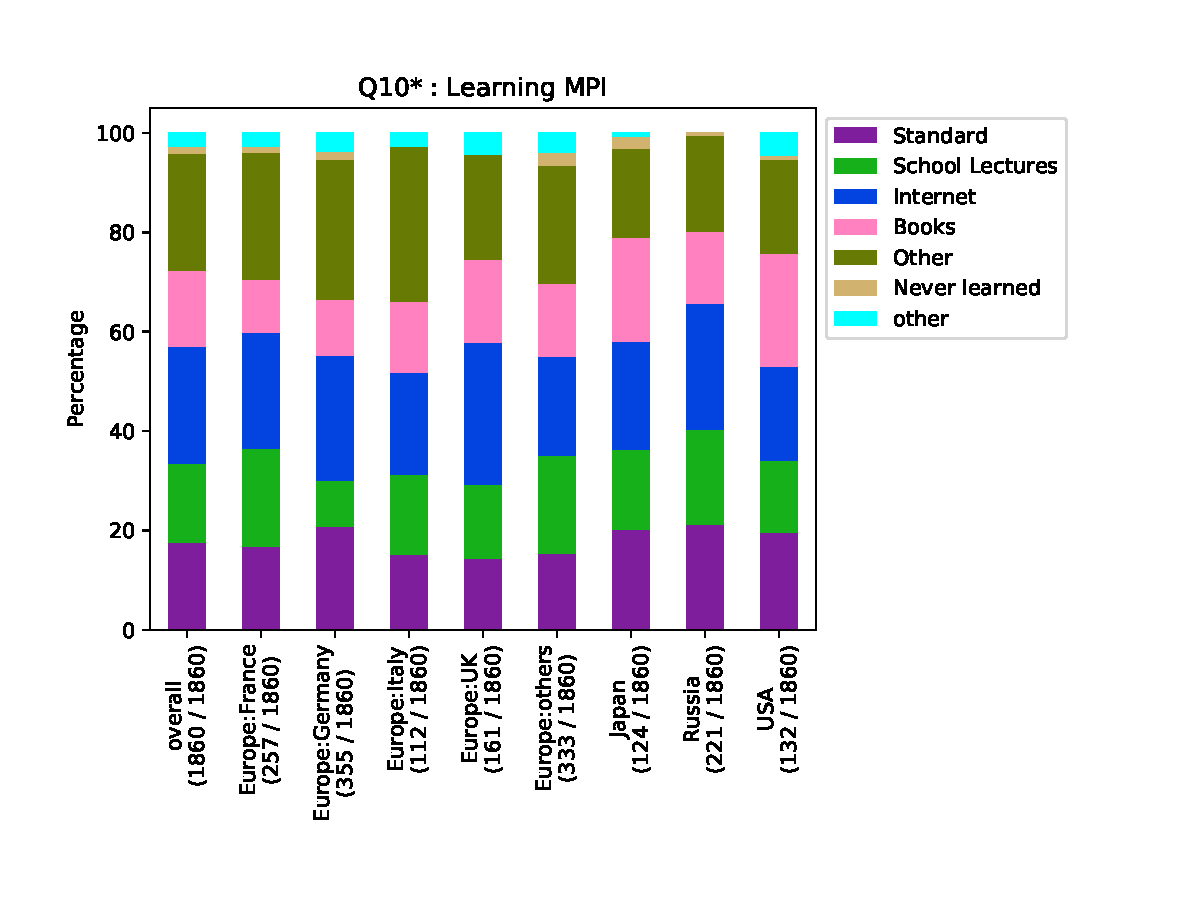
\includegraphics[width=10cm]{../pdfs/Q10.pdf}
\caption{Simple analysis: Q10}
\label{fig:Q10}
\end{center}
\end{figure}
